\documentclass[11pt]{article}

\date{}

\usepackage{fullpage}
\usepackage{graphicx}

\begin{document}

\title{Design Principles for Scalable Genomic Analysis Systems}
\author{Frank Austin Nothaft}
\maketitle

\abstract

Improvements in the throughput and cost of genomic sequencing techniques have made it practical to incorporate
sequencing assays into research and clinical practice. However, current analysis toolkits cannot achieve the latency
required for clinical work, nor the scale required for next-generation population genomics studies. By using the
computational frameworks that have been developed for large-scale data analytics, we can design processing
pipelines that achieve our latency/throughput goals by scaling across several hundred computers. 

\section{Introduction}

\begin{enumerate}
\item Introduction
\begin{enumerate}
\item Application
\begin{enumerate}
\item End-to-end pipeline for genomic analysis:
\begin{itemize}
\item Input: raw reads from sequencer output
\item Align reads to reference genome
\item Process reads to de-skew data
\item Call variants
\end{itemize}
\item Variant call outputs are important in clinical use, and for population-level analysis
\begin{itemize}
\item Variant calls describe distribution of alleles in population, as well as genotypes of individuals
\item Majority of called variants are single nucleotide polymorphisms (SNPs)
\item We are also interested in calling short insertions/deletions (INDELs) and copy number variations (CNVs, the duplication of a gene)
\end{itemize}
\item End-to-end latency is $>$50 hrs for current systems, this is highly limiting for clinical analysis
\begin{itemize}
\item Sub-24hr latency is required for personalized medicine
\item Pipeline latency also limits throughput of sequencing assays on populations
\end{itemize}
\end{enumerate}
\item Aims
\begin{enumerate}
\item Develop a pipeline that can perform this processing end-to-end in one hour
\item Use distributed computing frameworks to make a system that can easily be scaled to hundreds of computers
\item Develop software under non-viral open source license to enable acceptance and use
\end{enumerate}
\end{enumerate}
\item Related Work
\begin{enumerate}
\item Computational Frameworks
\begin{itemize}
\item Spark
\item Parquet
\item Avro
\end{itemize}
\item Variant Calling Frameworks
\begin{itemize}
\item Genome Analysis Toolkit (GATK)
\item SAMTools
\item Short Oligonucleotide Analysis Package (SOAP)
\item FreeBayes
\end{itemize}
\end{enumerate}
\end{enumerate}

\section{Architecture}

\begin{enumerate}
\item Scalable analysis pipeline in Spark on top of ADAM---see fig. \ref{fig:architecture}
\item Alignment
\begin{enumerate}
\item Alignment performed using SNAP using genome index
\item Alignment is distributed across $n$ nodes inside of SNAP framework
\item Use interleaved FASTA input format to simplify division/streaming
\item To keep data from touching disk, open streams to/from SNAP
\end{enumerate}
\item Preprocessing
\begin{enumerate}
\item Preprocessing serves to eliminate latent biases in reads
\item Preprocessing done using ADAM, described in \S\ref{sec:preprocessing}
\end{enumerate}
\item Variant Calling
\begin{enumerate}
\item Have implemented both pileup based and assembly calling methods
\item Support genomic region dependent processing methods---brief discussion of \textsc{CAGe} and SiRen
\item See \S\ref{sec:call}
\end{enumerate}
\end{enumerate}

\begin{figure}[h]
\begin{center}
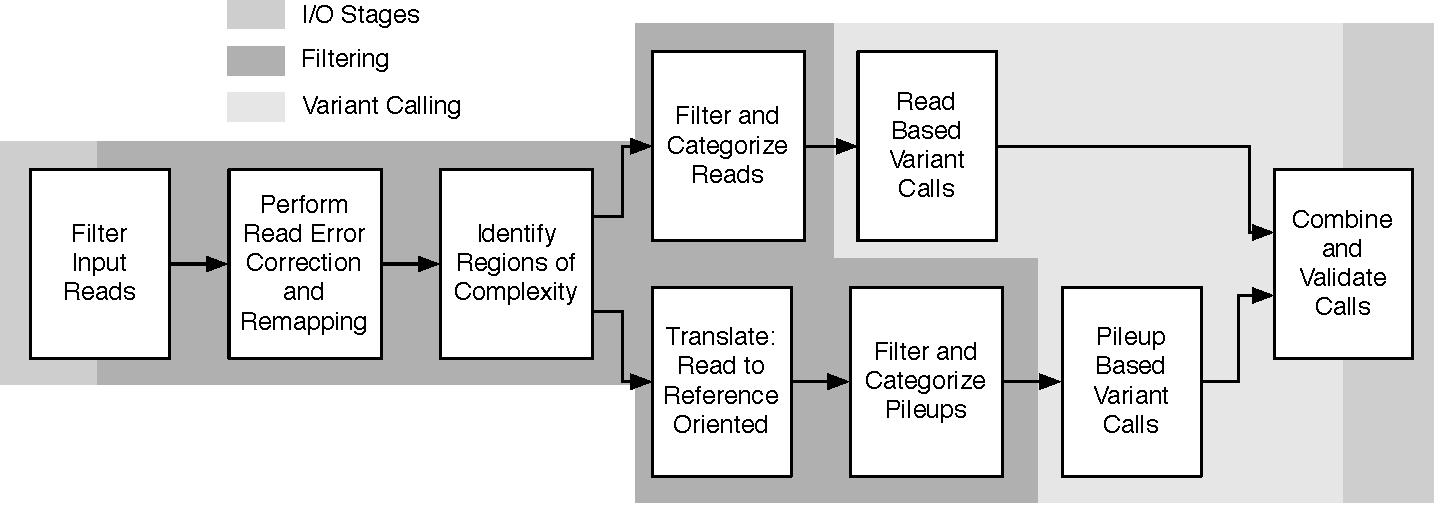
\includegraphics[width=0.9\linewidth]{avocado-architecture.pdf}
\end{center}
\caption{System architecture}
\label{fig:architecture}
\end{figure}

\section{Read Preprocessing Algorithms}
\label{sec:preprocessing}

\begin{enumerate}
\item Duplicate Marking/Removal
\begin{enumerate}
\item Goal is to remove PCR/optical duplicate reads
\item Mostly an issue for WES/target assays
\item Describe heuristics for identifying duplicate reads---TBA
\end{enumerate}
\item Indel Realignment
\begin{enumerate}
\item Short read alignment achieves correct global alignment but can have incorrect local alignment
\item Local realignment is a heuristic algorithm that cleans local alignments IFF an improvement in weighted Hamming distance can be achieved
\item Discuss different consensus sequence determination methods and impact on accuracy
\item Why is indel realignment needed when local assembly is available? Somatic variant calling.
\end{enumerate}
\item Base Quality Score Recalibration
\begin{enumerate}
\item TBA
\end{enumerate}
\end{enumerate}

In this section (and the section below), go through discussion of algorithms and performance characteristics for above algorithms. Characterize:

\begin{itemize}
\item Across datasets: WGS (with PCR/PCR-free for duplicate marking), WES, targeted, high/low coverage, somatic/germline
\item Across configuration parameters
\item Across dataset sizes
\end{itemize}

\section{Variant Calling Algorithms}
\label{sec:call}

\begin{enumerate}
\item Single Locus Calling
\begin{itemize}
\item Qualitative comparison of current method vs. Unified Genotyper/FreeBayes/mpileup
\item Discussion of internal EM algorithm for maximization
\item Discussion of impact of joint variant calling as coverage changes---compare to \textsc{CAGe++}
\end{itemize}
\item Local Assembly
\item Copy Number Variant calling---TBA
\end{enumerate}

\section{Discussion}

\begin{enumerate}
\item Comprehensive discussion of concordance/discordance between pipelines
\begin{itemize}
\item SNAP/\texttt{avocado}
\item SNAP/GATK
\item BWA-MEM/GATK
\item BWA-MEM/FreeBayes
\item SOAP suite
\end{itemize}
\item Future Work
\begin{itemize}
\item Somatic variant calling
\item Sufficient statistics/variant calling vs. database
\end{itemize}
\end{enumerate}

\end{document}